\chapter{Design Overview}\label{chap:design}

This chapter presents the details of the DADT/LN prototype implemented as part of
this work. The chapter begins with an outline of the limitations of the
existing DADT prototype \cite{migliavacca_DADT:2006}. This is followed by a
discussion on the architecture of the hybrid DADT/LN prototype that combines
the functionality of the DADT prototype with the LN routing mechanism, and
extends the existing prototype to work on WSNs.

\section{Limitations of the existing DADT Prototype}

The DADT prototype proposed in \cite{migliavacca_DADT:2006} enables the use of
DADTs to facilitate distributed application programming.

It supports Java-based application development, and consists of two parts:
\begin{itemize}
  \item \emph{Translator}
  \item \emph{Runtime library} 
\end{itemize}

The \emph{translator} translates Java programs
  extended with DADT programming constructs into conventional Java classes.

The \emph{runtime library} is used during the translation stage, and allows for
the execution of the Java classes in the J2SE. It provides support for DADT
constructions and methods, such as \emph{binding} ADTs to DADTs, \emph{DADT Views}, \emph{Actions} and
\emph{Operators}.

The communication in the prototype uses IP Multicast, and
allows the delivery of information to ADTs bound to a specific DADT\footnote{Group of ADTs of this kind are defined as
multicast groups in the prototype.}.

The DADT prototype is a proof of the DADT concept. While this
approach is clearly applicable to WSNs, the prototype itself did not support WSN
abstractions, as it suffers from the following major limitations:

\begin{itemize}
  \item The lack of a routing mechanism suited for WSN
  \item Limitations in portability to real WSN nodes
  \item Memory and code occupation
\end{itemize}

\section{The DADT/LN Prototype Design} \label{sec:PrototypeDesign}

The DADT prototype proposed in \cite{migliavacca_DADT:2006} proved that the
concept of DADTs could possibly be applied to WSN
applications, but existing limitations in the prototype prevent its use in WSN simulators or real nodes.

This work makes the following contributions:

\begin{itemize}
  \item Enhances the DADT prototype for use in WSNs by extending it to run
  on simulators as well as devices in a real-world environment.
  \item Interfacing the LN mechanism presented in \cite{mottola_LNAbstraction} with the DADT prototype in order
  to enable abstracted communication between groups of nodes in the WSN defined
  by DADTs.
  \item  Verifies the utility of DADT abstractions in the WSN
  application layer.
\end{itemize}

\subsection{Workflow Overview} \label{subsec:overview}
\begin{figure}
\centering
\includegraphics[width=\textwidth]{img/DADTLN_workflow.eps} 
\caption[DADT/LN application workflow]{Workflow for development of an application that uses
the DADT/LN prototype}
\label{Fig:DADTLN_workflow}
\end{figure} 
The overview of the workflow involved in using DADTs to enable WSN application
programming is shown in Figure \ref{Fig:DADTLN_workflow}. The application
developer writes the application layer code for the WSN  in a series of \emph{.dadt} files using the DADT
specification language. The JADT preprocessor is then used to convert the code written by the
application programmer into Java code that interfaces with the DADT infrastructure (extended from the prototype presented in \cite{migliavacca_DADT:2006}). In order to facilitate routing using LNs, the DADT infrastructure is interfaced with a
previously developed implementation of LNs \cite{mottola_LNAbstraction}. 

The application (including the implementation of layers lower in the protocol
stack) is then loaded on to either:
\begin{itemize}
\item the JiST/SWANS simulator \cite{barr_JIST:2005, barr_SWANS} (See Section
\ref{sec:jistswans} for the implementation details of the simulator) 
\item a collection of Sun SPOT wireless sensor devices
\cite{simon_squawk:2006} (see Section \ref{sec:sunspots}) to execute the given 
application on real sensor nodes.
\end{itemize}

\begin{figure}
\centering
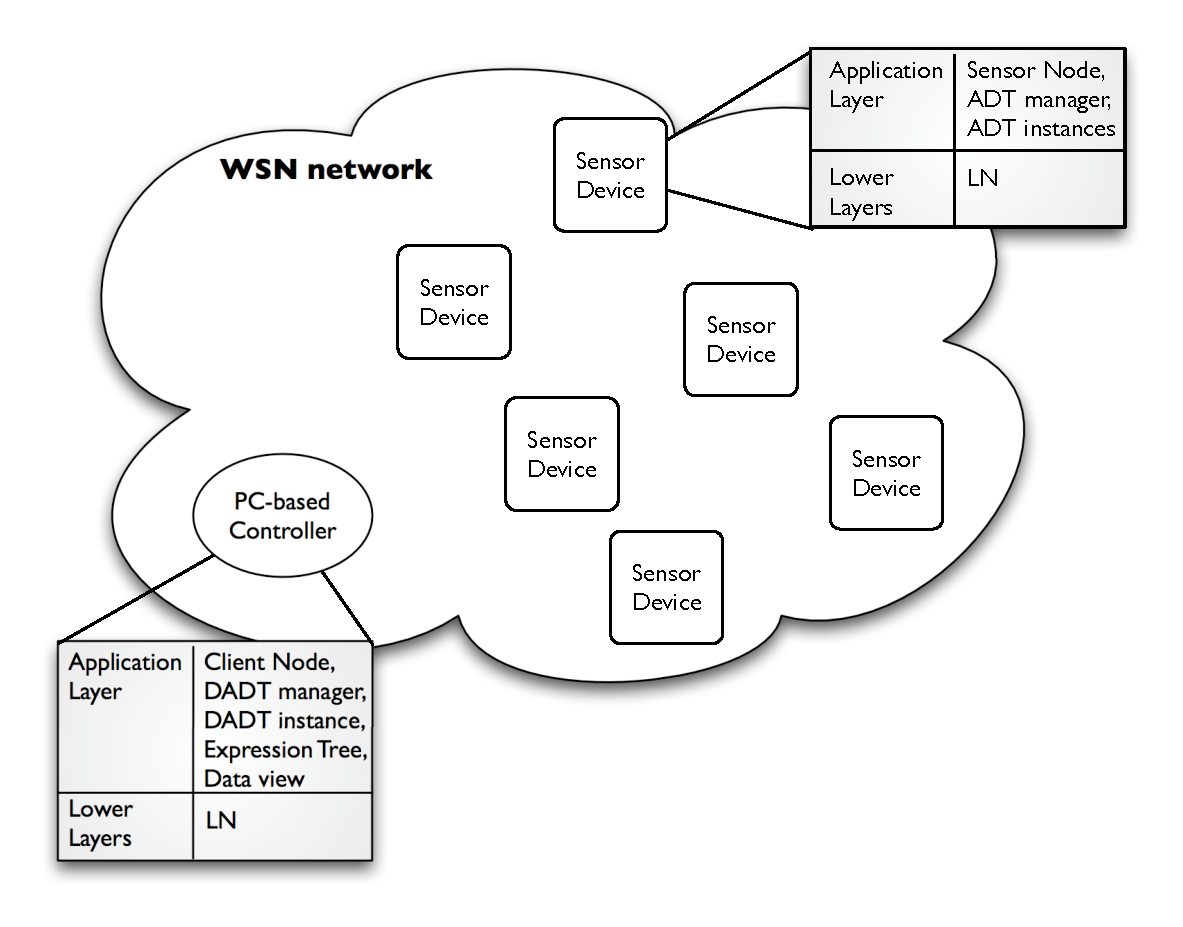
\includegraphics[scale=0.55]{img/DADTLN_glossary.eps} 
\caption[WSN in DADT/LN prototype]{Schematic representation of the WSN as
abstracted in the DADT/LN prototype}
\label{Fig:DADTLN_glossary}
\end{figure} 

The WSN in the DADT/LN prototype developed as part of
this work consists of two types of devices each of which conceal a number
of objects on the different layers of the WSN stack, as shown in Figure
\ref{Fig:DADTLN_glossary}:

\begin{itemize}
  \item \emph{DADT Controller Device}
  \item \emph{Sensor Device}
\end{itemize}  
   
\emph The {DADT Controller Device} can reside, depending on the
application, either on a real-world sensor device such as a Sun
SPOT, or be a PC-based application. On the application layer, this
abstraction includes the distributed application code, the DADT instance, and the DADT manager. The network layer entity hosts the LN implementation.
  
\emph The {Sensor Device} is a real-world sensor device such as a Sun SPOT, 
which holds the application layer entities, which includes a Sensor Node
abstraction consisting of multiple sensor ADT instances, and an ADT
manager, and a network layer entity represented by the LN implementation.

\subsection{Architecture}

The architecture of the DADT/LN prototype is presented in Figure
\ref{Fig:DADTLN_architecture}, and consists of the following logical layers.

\begin{figure}
\centering
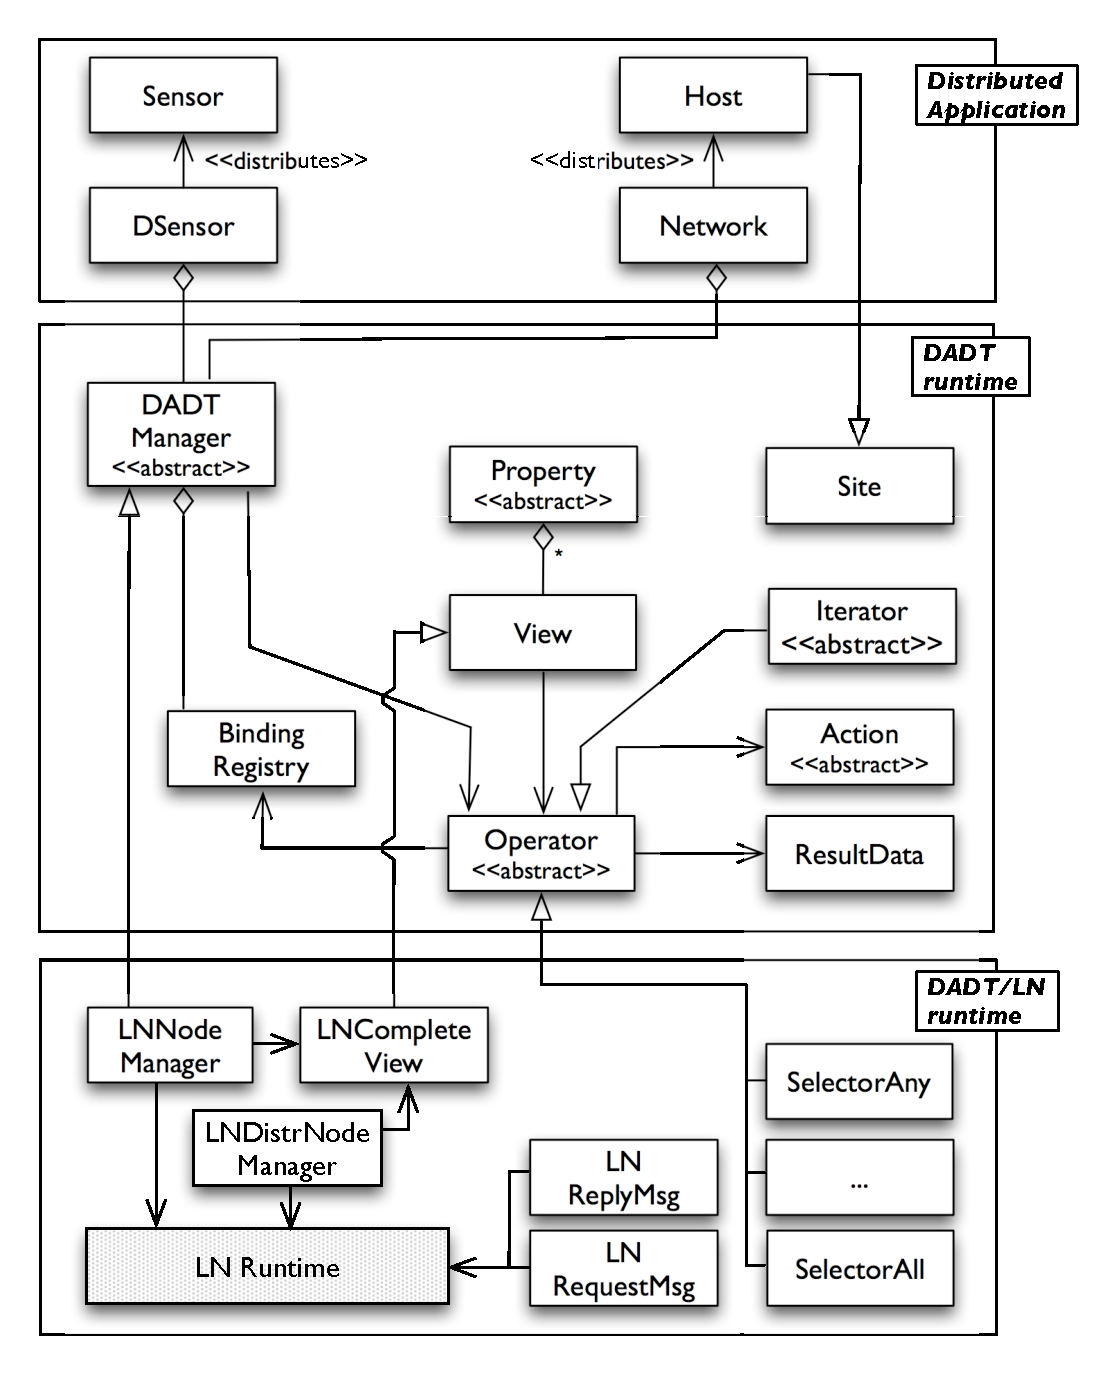
\includegraphics[scale=0.65]{img/DADTLN_architecture.eps} 
\caption[DADT/LN architecture]{Architecture of the DADT/LN prototype}
\label{Fig:DADTLN_architecture}
\end{figure} 

\subsubsection{Upper layer}

The upper layer consists of the following components:

\begin{itemize}
\item \emph {Distributed application}
\item \emph{Sensor} and \emph{DSensor}
\item \emph{DADT runtime layer}
\item \emph{DADT manager}
\item \emph{The Property, Action, and View classes}
\end{itemize}

The Distributed application comprises the code implemented by
the application developer, and is written in the DADT specification language. This code is later  translated into executable Java
code using the JADT preprocessor, and interfaced with the DADT runtime (see Section \ref{subsec:overview}).

The \emph{Sensor} and \emph{DSensor} classes are the data ADT and data DADT
specifications used by the DADT/LN prototype, and are entirely defined by the
application developer. The space ADTs \emph{Host} and \emph{Network} are
currently built into the DADT/LN prototype, and cannot be defined by the
application programmer. 

The \emph{DADT runtime layer} holds the DADT runtime library, which provides
handling of ADTs and DADTs. 

The \emph{DADT Manager} performs several tasks, including managing the binding and unbinding
of ADT instances to DADT type by means of the  \emph{Binding Registry} class,
and providing support for space ADTs using the \emph{Site} class. 

The abstract classes \emph{Property} and \emph{Action} represent the
corresponding concepts described in Section \ref{subsec:DADTsConcepts}.
The class \emph{View} provides support for data and space DADT Views, and
contains the set of \emph{Property} objects that define the scope of the
operations. 

Properties are organised into an abstract tree that codifies the
logical predicates defining the view, with the leaves representing DADT
properties and the nodes specifying boolean operators that are used to compose it.
The class \emph{Operator} is a superclass for all of the DADT Operators, though
the current implementation of the DADT/LN prototype provides support mainly for
selection operators.

\subsubsection{Lower Layer} \label{subsubsec:LowerLayer}

The \emph{DADT/LN runtime} layer provides support for interfacing the DADT
runtime with the LN runtime \footnote{The LN implementation
used as part of this work does not use a declarative language for LN
specification which was used for decription of the LN concepts}, which enables
routing and scoping mechanisms in WSN. 
Interaction with LN runtime achieved by using instances of
the \emph{LNNodeManager} class on each sensor device, and the \emph{LNDistrNodeManager} instance on the controller node.

Communication between sensor devices and the controller node is fully handled by
the LN runtime layer. This is abstracted from the application programmer by means of the
\emph{Request} and \emph{Reply} messages (details of implementation are provided
in Section \ref{sec:messages}). The classes \emph{SelectAll} and \emph{SelectAny} implement
DADT selection operators, and allow for the invocation of the corresponding send methods defined in the LN API.

\section{Summary}

This chapter presented the architecture of the DADT/LN
prototype developed during the course of this work. The chapter concluded with a
detailed description of the modules constituting the prototype and 
interaction between them.
